
%%%%%%%%%%%%%%%%%%%%%%% file typeinst.tex %%%%%%%%%%%%%%%%%%%%%%%%%
%
% This is the LaTeX source for the instructions to authors using
% the LaTeX document class 'llncs.cls' for contributions to
% the Lecture Notes in Computer Sciences series.
% http://www.springer.com/lncs       Springer Heidelberg 2006/05/04
%
% It may be used as a template for your own input - copy it
% to a new file with a new name and use it as the basis
% for your article.
%
% NB: the document class 'llncs' has its own and detailed documentation, see
% ftp://ftp.springer.de/data/pubftp/pub/tex/latex/llncs/latex2e/llncsdoc.pdf
%
%%%%%%%%%%%%%%%%%%%%%%%%%%%%%%%%%%%%%%%%%%%%%%%%%%%%%%%%%%%%%%%%%%%


\documentclass[final,a4paper]{llncs}
%\usepackage[spanish]{babel}
\usepackage{amssymb}
\setcounter{tocdepth}{3}
\usepackage{graphicx}
\usepackage{url}
\usepackage%[disable] %% descomentar para borrar o dejar de mostrar las notitas de colores
{todonotes}
%%%> paquetes y seteo de tikz figures
%\usepackage{tikz}
\usepackage{verbatim}
%\usepackage[active,tightpage]{preview}
%\PreviewEnvironment{tikzpicture}
%\setlength\PreviewBorder{5pt}%
%%%>
%\usetikzlibrary{arrows}
%% The lineno packages adds line numbers. Start line numbering with
%% \begin{linenumbers}, end it with \end{linenumbers}. Or switch it on
%% for the whole article with \linenumbers after \end{frontmatter}.
\usepackage{lineno}
%tildes y otros simbolos del español
\usepackage[utf8]{inputenc}
% simbolo INDEPENDENCIA probabilistica
\newcommand{\indep}{\rotatebox[origin=c]{90}{$\models$}}

\newcommand{\degree}{$^{\circ}$}

\urldef{\mailsa}\path|{ana.diedrichs,facundo.bromberg
}@frm.utn.edu.ar| 
\newcommand{\keywords}[1]{\par\addvspace\baselineskip
\noindent\keywordname\enspace\ignorespaces#1}

\begin{document}

\mainmatter  % start of an individual contribution

% first the title is needed
\title{Modelo de balance calórico de heladas}
% Exploring sensor temperature relationships in order to improve the prediction

% a short form should be given in case it is too long for the running head
\titlerunning{modelo de difusión de calor}

% the name(s) of the author(s) follow(s) next
%
% NB: Chinese authors should write their first names(s) in front of
% their surnames. This ensures that the names appear correctly in
% the running heads and the author index.
%
\author{Ana Laura Diedrichs
%\and Facundo Bromberg
}
%
\authorrunning{}

% (feature abused for this document to repeat the title also on left hand pages)

% the affiliations are given next; don't give your e-mail address
% unless you accept that it will be published
\institute{Laboratorio DHARMa, Dpto Sistemas, \\
Facultad Regional Mendoza, Universidad Tecnol\'{o}gica Nacional,\\
Rodríguez 273, Ciudad de Mendoza, Argentina, 5500\\
\mailsa\\
%\mailsb\\
%\mailsc\\
\url{http://dharma.frm.utn.edu.ar}
}

\toctitle{Lecture Notes in Computer Science}
\tocauthor{Authors' Instructions}
\maketitle


%%
%% Start line numbering here if you want
%%
\linenumbers

\begin{abstract}

ESCRIBIR LUEGO

\end{abstract}

\section{Problemática de las Heladas}

Las heladas constituyen uno de los accidentes de tiempo que causan grandes pérdidas 
económicas, a la agricultura en la Argentina y gran parte del mundo, e impacto
social al verse afectado los cultivos de los productores, debido a que no son fenómenos 
locales sino extensivos. Existen varias definiciones de helada como considerar helada a las 
temperaturas mínimas menores a 0\degree C. La más apropiada desde el punto de vista agronómico
es \emph{considerar a la helada como el evento meteorológico que ocurre cuando los cultivos 
y otras plantas experimentan daño por congelación}. El daño causado por heladas ocurre 
cuando las temperaturas están debajo de un límite tolerable para
los cultivos. El umbral de resistencia de las plantas al frío varía de acuerdo 
al estado fenológico en el que se encuentren (floración, frutos o yemas presentes, etc) 
%TODO CITAR TRABAJO CHAAR %\cite{snyder2005frost}. 
Según el Instituto Nacional de Vitivinicultura (INV) en el 2013 la pérdida de viñedo por
helada llegó a un 27\% \cite{inv-news}. Las heladas tardías en Mendoza suceden entre septiembre y noviembre
siendo muy peligrosas porque empieza la floración y ya hay yemas brotadas. 

\begin{figure}[h]
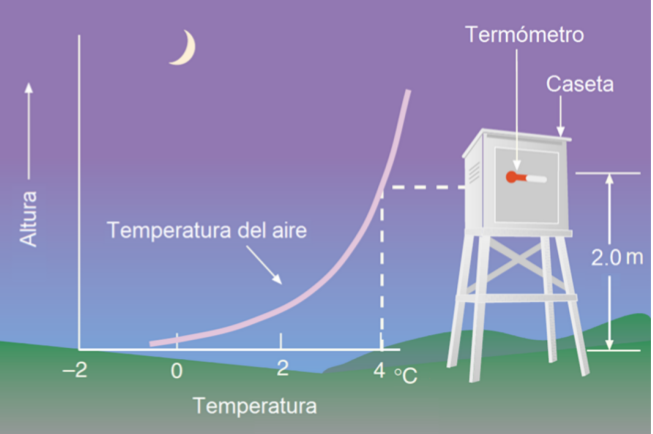
\includegraphics[width=0.70\columnwidth]{casilla.png}
\end{figure}\label{fig:casilla}

Existen dos tipos de heladas. Las heladas advectivas se caracterizan por los
 altos niveles de humedad, escarcha y cielo nublados. Las heladas radiativas suceden 
 bajo cielo despejado, escaso viento y muy baja humedad. Estas últimas son consideradas muy peligrosas
 porque el balance calórico disminuye drásticamente en la noche despejada al perderse el 
 calor recibido durante el día. Para la medición de variables ambientales comúnmente se utilizan estaciones meteorológicas. Actualmente las mismas están instaladas muy distanciadas unas de las otras, por lo que no son suficientes para 
caracterizar un fenómeno micro-climático. A esto se suma que la casilla meteorológica está
a una altura promedio entre los 1.5m y 2m, como lo ilustra la figura\cite{saavedraTesis} anterior; impidiendo
 caracterizar el fenómeno de la inversión térmica. En el siguiente gráfico \cite{pid-fca-uncu-dataset}
 se muestran las temperaturas durante una noche de heladas de seis sensores 
posicionados verticalmente (a nivel del suelo, 40cm, 75 cm, 1.5m, 2 m, 3 m) donde 
podemos visualizar la variabilidad de la amplitud térmica a distintas alturas. 
Esto sucede porque el aire frío es más denso y fluye hacia las capas más bajas, 
en consecuencia drena hacia la parte más baja del terreno; mientras que 
el aire más caliente queda estratificado en la 
altura. Por esto es importante medir la variable de interés (temperatura) in situ y a distintas
alturas.
La predicción de heladas es importante porque permite activar con tiempo los mecanismos de 
prevención activa. Durante las noches de heladas suelen utilizarse quemadores, molinos de viento,
aspersores, entre otras técnicas que permiten generar o mejorar la circulación del calor donde 
se encuentran los cultivos. Por otra parte, la predicción localizada de heladas permitiría 
saber no sólo si helará o no ese día,
sino también las zonas de una finca o región que se verían afectadas.

\begin{figure}[h]
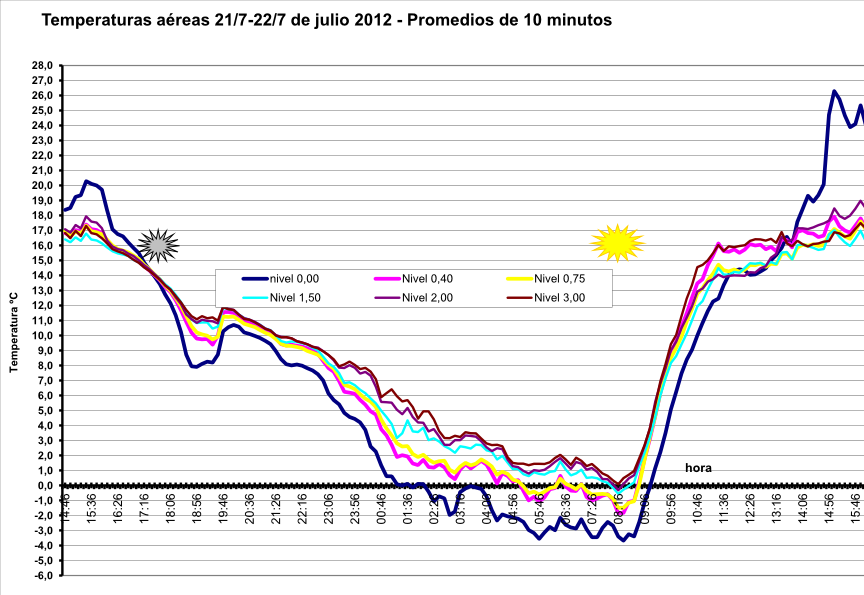
\includegraphics[width=0.99\columnwidth]{grafico.png}
\end{figure}\label{fig:T3-result}

\section{Balance calórico de una noche de helada}

 El descenso térmico que caracteriza una noche de helada está determinado por un balance calórico negativo
 del entorno. Intervienen varias causas de pérdida del calor del sistema que denominaremos como flujos salientes
 o entrantes cuya unidad es $W/m^2$ (watts por metro cuadrado).
 
 Los elementos que componen el balance calórico están determinados por la ecuación fundamental que describe 
 el proceso:
 
$$Q_G + SH + LH + Q^*+S_C=0$$

En las noches de heladas el ambiente se enfría, ocasionando que el suelo pierda el calor adquirido durante
el día gracias al sol. El flujo por conducción en el suelo ($Q_G$) es el flujo de energía desde el subsuelo a la superficie
(positivo) y viceversa (negativo). Este flujo de calor por conducción del suelo se puede cuantificar
usando la ley de Fourier, que indica que el calor $Q_G$ es proporcional al gradiente de temperatura
(primera ley de conducción del calor): 

$$Q_G=-k* Area * \nabla T $$. 

La constante $k$ es la conductividad térmica del suelo.
El gradiente de temperatura que representa el flujo de calor entre suelo y ambiente se caracteriza como la siguiente fórmula 
$\nabla T =\frac{dT}{dt}=\frac{dT}{dx}+\frac{dT}{dy}$. Dada la presencia de derivadas parciales, la misma se resolverá 
mediante diferencias finitas y considerando dimensiones 2D para simplificar el problema.


El flujo de calor sensible $SH$ está asociado a la diferencia de temperatura que existe entre la temperatura
a nivel de superficie y la temperatura a nivel de aire. Su valor es positivo si la energía fluye 
desde el aire hacia la superficie y negativo en caso contrario. Se calcula como 
$SH=C_H*\overline{W}*(\overline{T}-T_G)$, siendo
$W$ la velocidad promedio del viento, $T$ la temperatura a nivel del aire, 
$T_G$ la temperatura a nivel del suelo, y $C_H$ es un coeficiente que en condiciones de estabilidad
puede variar entre $10^{-3}$ a $5*10^{-3}$. Se considera que $\overline{T}-T_G = \nabla T $, es decir,
reemplazar la expresión por el gradiente de temperatura quedaría determinada como
$$SH=C_H*\overline{W}*\nabla T$$

El flujo de calor latente ($LH$) está asociado con los cambios de fase del agua, es decir, cuando hay 
evaporación o condensación sobre la superficie del suelo. Se calcula como
$$LH=C_E*\overline{W}*(\overline{q}-q_G)$$, siendo $q$ la humedad del aire, $q_G$ la humedad relativa a
nivel del suelo, y $C_E$ un coeficiente de estabilidad similar a $C_H$. Dado que esta ecuación representa 
el aporte/sustracción ante los cambios de estado del agua; al interesarnos simular una situación de helada
puede calcularse $LH$ en el caso de que la temperatura sea menor o igual a cero,
porque el agua cambia a estado sólido; de lo contrario $LH=0$.

El flujo por radiación neta ($Q^*$) considera la suma de la radiación emitida/recibida en los dos rangos
espectrales: radiación de onda corta (SW) y radiación de onda larga. Durante una noche de helada, dada
la ausencia de radiación solar, la ecuación se simplifica considerando sólo la radiación de onda larga.
$$ Q^*=LW \downarrow - LW \uparrow $$
$LW \downarrow$ es el flujo de onda larga que el suelo recibe y es emitida casi en su totalidad por toda la 
atmósfera, dependiente de la temperatura, humedad y cobertura nubosa. Las nubes juegan
un papel muy importante durante la noche ya que modulan la temperatura de la superficie mediante la emisión
radiación infrarroja. 

$LW \uparrow$ representa el flujo
de radiación de onda larga emitida desde la superficie terrestere hacia la atmósfera por lo que depende
de la temperatura del suelo y su emisividad. Interesa señalar que es responsable del calentamiento
y enfriamiento del aire, debido a que el aire no absorve la radiación solar por ser de onda corta, pero 
sí absorbe la del suelo que es onda larga. Está regida por la ley de Stefan-Boltzmann 
$LW \uparrow = \epsilon * \sigma * T_G^4 $, donde $\epsilon$ es el coeficiente de emisividad del suelo, 
$\sigma = 5.67 * 10^{-8} \frac{J}{m^2 s K}$ la constante de Stefan-Boltzmann y $T_G$ la temperatura en grados
Kelvin del suelo.

El flujo de calor por convección varía proporcionalmente según la constante de convección, definimos
$S_C = h * \nabla T$

\section{Simplificaciones del modelo} 
\begin{itemize}
\item El problema se simplificará analizando la difusión del calor en el suelo y luego en el aire unidimensionalmente.
\item La capacidad térmica y emisividad del suelo no variará con el tiempo.
\item En la noche no hay radiación solar presente y la misma ha sido absorvida por el suelo durante el día
\item Se analizará la variación de la temperatura en el tiempo, según condiciones de frontera iniciales 
(por ej. temperatura a nivel subsuelo, temperatura a nivel suelo)
\end{itemize}
\section{Difusión del calor en el suelo}
 Evaluar la variación de la temperatura del suelo de acuerdo a la difusión del calor desde el subsuelo al suelo,
 presentado como: $Q_G=-k* Area * \nabla T $. Para empezar a codificar y simular el comportamiento usando R , 
 utilizamos la librería ReacTran [1]. Esta librería cuenta con rutinas para el desarrollo de modelos de 
 reacción y transporte, con advección 
 y difusión en una, dos o tres dimensiones. Principalmente provee:
\begin{itemize}
\item Funciones que subdividen el espacio en un número discreto de celdas en una grilla
\item Aproximación por diferencias finitas o volúmenes finitos del término de transporte advectivo-difusivo
\end{itemize}

 $$ \frac{\partial T}{\partial t}
 = -\frac{1}{A_x\xi_x} \left( \frac{\partial}{\partial x} A_x
           ( -D \frac{\partial \xi_x T}{\partial x} ) - 
            + \frac{\partial}{\partial x} (A_x\, v\,  \xi_x\, T) \right) $$

En la fórmula anterior $D$ es el coeficiente de difusión, $v$ la tasa de advección, $A_x$ el área de la superficie y
$\xi$ la fracción de volumen. Considerando que $A$,$\xi$,$D$ y $v$ son constantes en x, la fórmula podría ser reescrita como:

 $$ \frac{\partial T}{\partial t} =  -D \frac{\partial^2 T}{\partial x^2}  - u
            \frac{\partial T}{\partial x}  $$

 Podemos observar que en el primer término tenemos una derivada de segundo orden y el segundo de primer orden. El
 primer término representa la tasa de difusión y el segundo término la tasa de consumo.
 Vamos a simular la propagación del calor desde el subsuelo al suelo basados en la siguiente fórmula:
 $$Q_G=-k* Area * \nabla T$$

\bibliographystyle{plain} %TODO <--- chequear que tome este estilo de bibliografía
\bibliography{references}

\end{document}
